\lhead{\emph{Theoretical Framework}}
\chapter{Theoretical Framework}

To achieve our goal of creating a multiresolution representation for neural media, we need to understand foundational concepts related to digital media representation, multiresolution theory, and neural networks. In the next sections, we provide an overview of signal processing and deep learning knowledge to familiarize the reader with the methods employed in our approach.


\section{Media Objects as Signals}

In a broad sense, a \textbf{signal} is a mathematical function that conveys information about a phenomenon. Signals can vary over time, space, or other domains, depending on the nature of the data being represented. Formally, a signal can be defined as a function \( f: \mathcal{D} \to \mathcal{C} \), where:

\begin{itemize}
  \item \( \mathcal{D} \) is the signal natural domain, representing time, space, or another variable.
  \item \( \mathcal{C} \) is the codomain, representing the values or attributes of the signal, such as intensity or color.
\end{itemize}

For example, an audio signal can be described as a function \( f(t): \mathbb{R} \to \mathbb{R} \), where \( t \) represents time and \( f(t) \) provides the amplitude of the sound wave at each moment. Similarly, an image can be interpreted as a two-dimensional signal \( f: U \subset \mathbb{R}^2 \to \mathcal{C} \) that maps spatial coordinates, a subset of the 2D Euclidean space, to color values. 

For an image to be precisely defined, we must provide a mathematical model for color. Typically, $\mathcal{C}$ is a subspace of $\mathbb{R}^3$. For instance, in the \textbf{RGB color model} each point \( (x, y) \) in the image maps to a vector \( (R, G, B) \) representing the intensities of red, green, and blue. Alternatively, in the \textbf{HSV color model}, the color space is parameterized by hue (H), saturation (S), and value (V), which provides a more perceptually intuitive representation of colors. For a detailed discussion on mathematical models for colors, please refer to \cite{ipcgVelho2014}.


A 3D surface can also be interpreted as a signal. This is often done by representing the surface implicitly as a level set of a scalar field. Specifically, an \textit{implicit surface} is defined by a function \( f : \mathbb{R}^3 \rightarrow \mathbb{R} \), where for any point \( \mathbf{x} = (x, y, z) \in \mathbb{R}^3 \), the function returns a scalar value encoding the \textit{signed distance} or a similar measure from the surface. The surface itself is the zero level set of the \textbf{implicit function} \( f(\mathbf{x}) \), that is, the set of points where this function evaluates to zero:

\[
\mathcal{S} = \{ \mathbf{x} \in \mathbb{R}^3 \mid f(\mathbf{x}) = 0 \}
\]

Points where \( f(\mathbf{x}) < 0 \) are inside the surface, and those where \( f(\mathbf{x}) > 0 \) are outside. For instance, a sphere of radius \( r \) centered at the origin is described by the implicit function:

\[
f(\mathbf{x}) = \|\mathbf{x}\| - r
\]

Interpreting \textbf{media objects} such as audio, images, and 3D models as signals is a natural and powerful approach because it allows us to apply established mathematical frameworks from signal processing. By treating these objects as signals, we can leverage techniques such as sampling, filtering, and reconstruction to model, analyze, and manipulate them.

% ### Graphical Objects as Signals

% Media objects can be modeled mathematically as signals by considering their structure and attributes. Following the formalism of \cite{gomesGraphical1996}, a graphical object \( \mathcal{O} \) is defined as a pair \( (\mathcal{U}, f) \), where:

% \begin{itemize}
%   \item \( \mathcal{U} = \{U_1, \dots, U_m\} \), with each \( U_i \subset \mathbb{R}^n \), is a collection of subsets of a Euclidean space \( \mathbb{R}^n \) that defines the \textit{geometric data set} of the object.
%   \item \( f: U_1 \cup \dots \cup U_m \to \mathbb{R}^p \) is the \textit{attribute function}, which assigns values (such as color, texture, or other physical properties) to each point in the geometric data set.
% \end{itemize}

% In this formalism, the domain \( U = U_1 \cup \dots \cup U_m \) defines the shape of the object, while the attribute function \( f \) assigns the object's properties. This perspective aligns well with interpreting media objects as signals, where the geometric structure corresponds to the domain, and the attributes of the object correspond to the signal values.


% #### Video as Signals

% A video can be viewed as a sequence of images evolving over time, making it a three-dimensional signal. It can be represented as a function \( f(x, y, t): \mathbb{R}^2 \times \mathbb{R} \to \mathcal{C} \), where \( (x, y) \) represents spatial coordinates, \( t \) is the time dimension, and \( \mathcal{C} \) is the color space. Each frame of the video corresponds to a 2D slice of the signal at a particular time.

% \[
% f(x, y, t) = \text{color at pixel } (x, y) \text{ at time } t
% \]

% This interpretation allows us to analyze both spatial and temporal aspects of the video signal, applying techniques such as spatiotemporal filtering, frame interpolation, and video compression.


\section{Overview of Signal Processing Theory}

\subsection{Sampling and Reconstruction}

Due to the finite nature of computational systems, continuous signals and objects must be discretized and stored in finite data structures. While certain media objects can be described through continuous mathematical models, such as vector graphics and other parameterized representations, these are less frequently employed for most practical purposes due to computational complexity or dificulty in modeling.

\textbf{Sampling} is the process of converting a continuous signal into a discrete sequence of values. One way this is accomplished is by measuring the signal's amplitude at specific intervals uniformly distributed in time and/or space, where the distance between consecutive measurements is known as the \textit{sampling rate}.

Discrete representations are easy to store and map to data structures; however, many operations—such as resizing, rotation, or resampling of the signal—require us to work with the continuous form of the signal. In such cases, the challenge lies in accurately reconstructing the continuous signal from its discrete samples. Figure \ref{f:sampling-reconstuction} illustrates the uniform sampling and reconstruction of a one-dimensional signal.


\begin{figure}[!h]
  \centering
  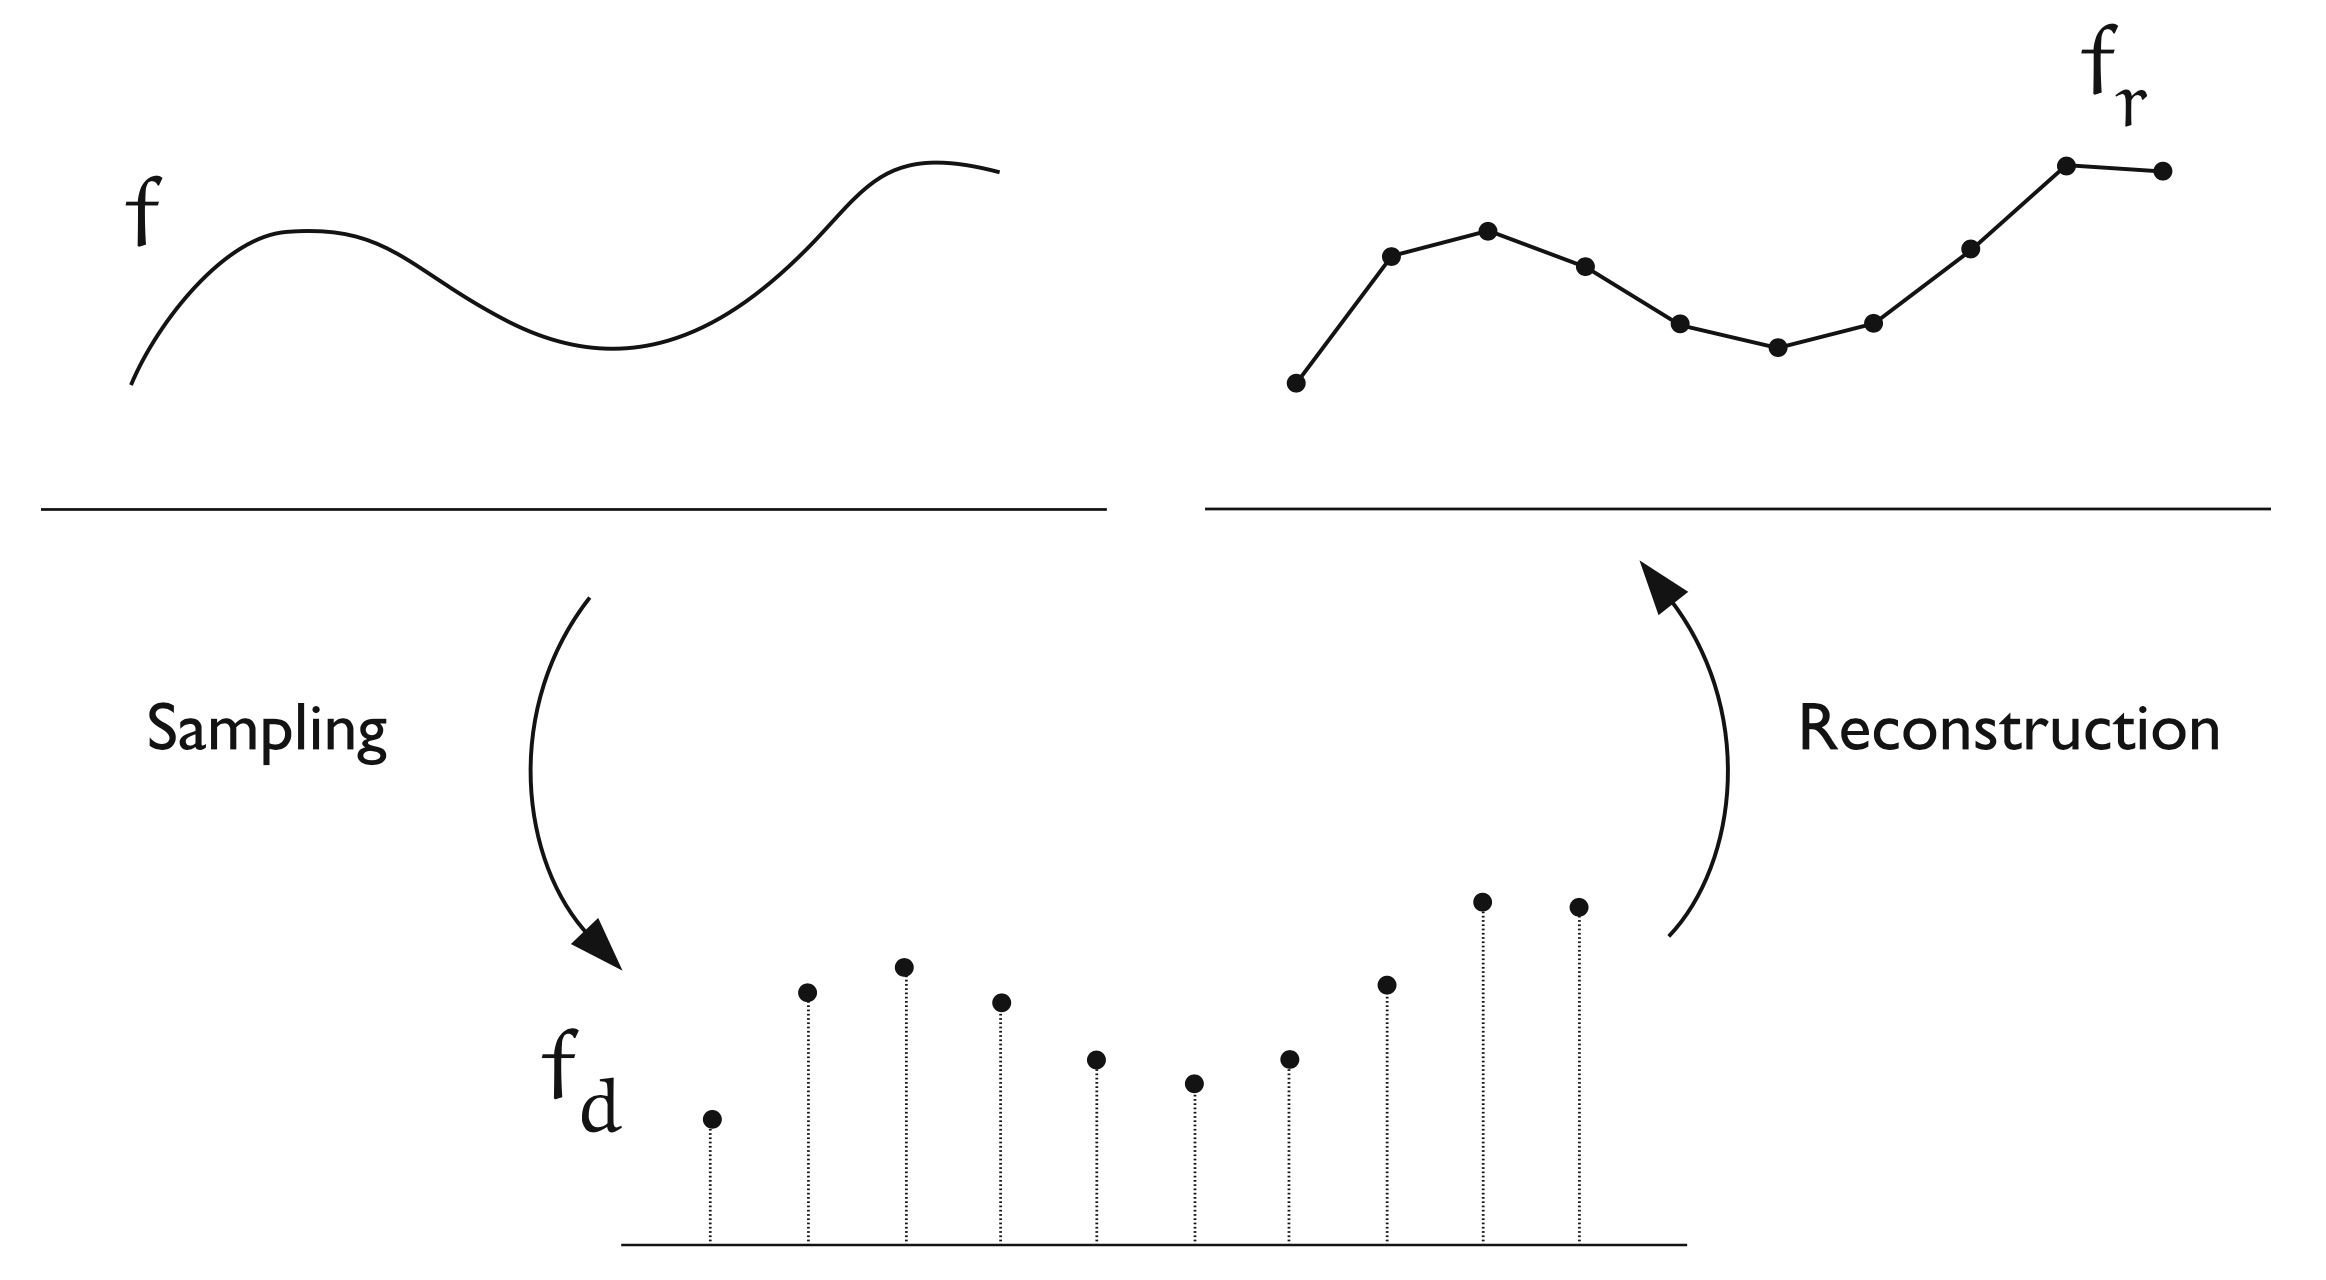
\includegraphics[width=0.85\linewidth]{img/ch2/sampling-reconstruction.png}
  \caption{Illustration of sampling and reconstruction processes (\cite{ipcgVelho2014}).}
  \label{f:sampling-reconstuction}
\end{figure}


One of the fundamental results in this area is the \textbf{Shannon-Nyquist Sampling Theorem} (\cite{Shannon1949}). This theorem asserts that a continuous-time, band-limited signal can be perfectly reconstructed from its samples, provided that the sampling rate is at least twice the highest frequency present in the signal. Formally, for a continuous-time signal \( f(t) \) with a maximum frequency component of \( B \) Hz, perfect reconstruction is possible if the sampling frequency \( F_s \) satisfies:
\[
F_s \geq 2B
\]

\begin{itemize}
  \item \( F_s \): Sampling frequency (in samples per second)
  \item \( B \): Maximum frequency of the signal (in Hz)
\end{itemize}

This theorem is central to digital signal processing, as it guarantees that we can reconstruct a continuous signal from a sufficient amount of samples under certain conditions. The critical threshold \( 2B \) is known as the \textbf{Nyquist frequency} or Nyquist limit. When the sampling frequency falls below the Nyquist limit, \textbf{aliasing} occurs. Aliasing is a form of signal distortion where higher frequency components are misrepresented as lower frequencies in the discrete signal. This distortion results in an inaccurate and misleading reconstruction of the original signal, as illustrated in Figure \ref{f:aliasing-example}.

\begin{figure}[!h]
  \centering
  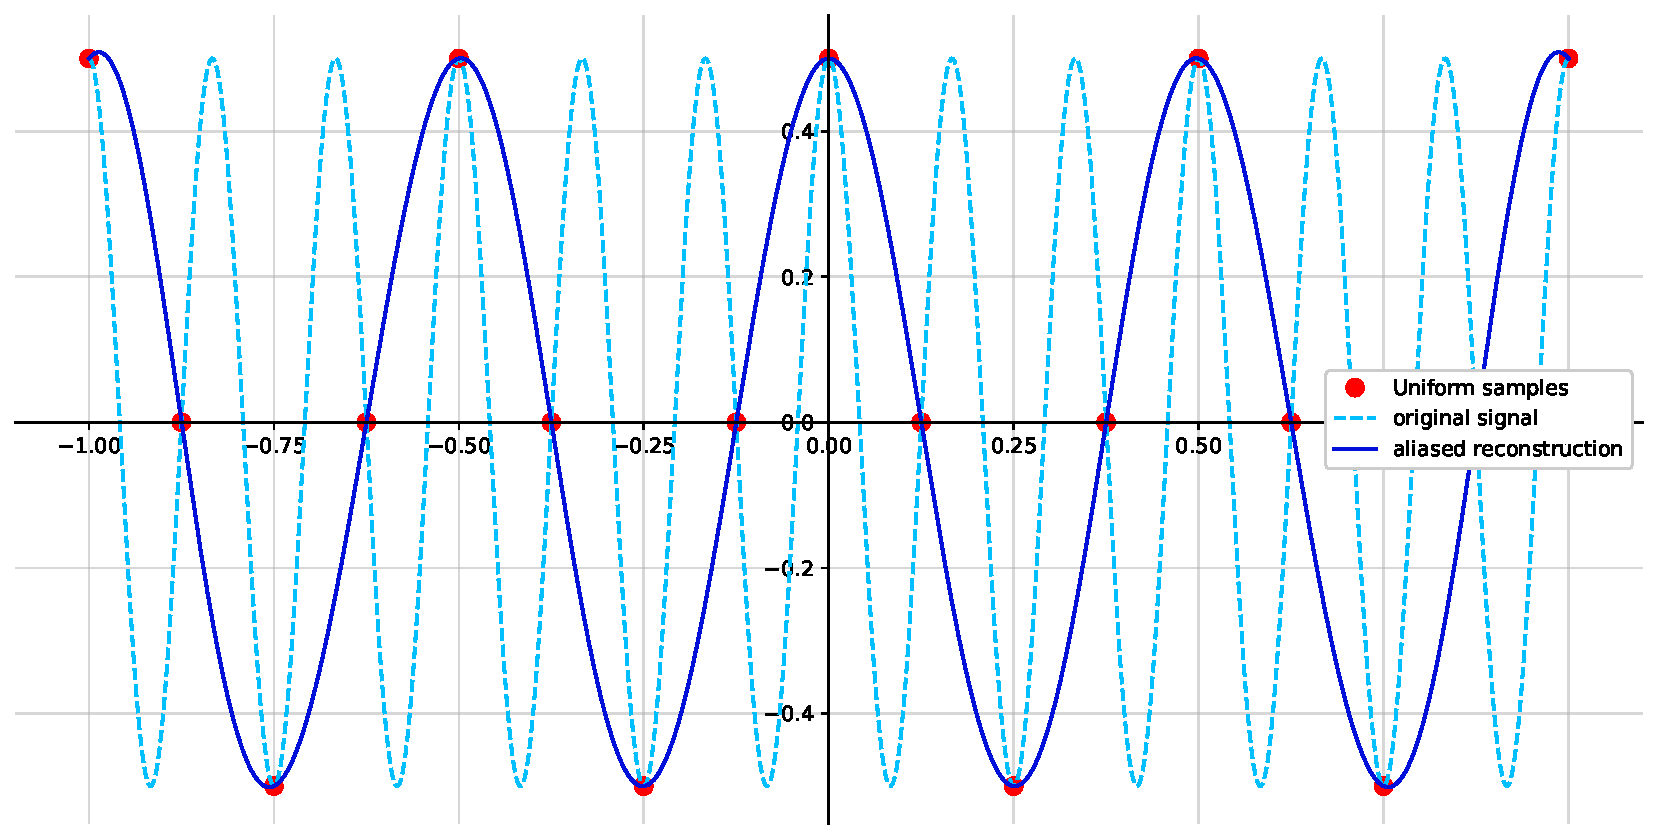
\includegraphics[width=0.85\linewidth]{img/ch2/aliasing-signal.pdf}
  \caption{Illustration of Aliasing.}
  \label{f:aliasing-example}
\end{figure}

Note that the Shannon-Nyquist theorem applies to \textbf{band-limited} signals—those whose frequency content is confined within a finite range. If a signal contains infinite frequency components, no finite sampling rate can fully capture its information. In such cases, even a high sampling rate would still result in aliasing, as the unbounded frequency components would fold into the baseband and distort the signal during reconstruction.

The process of signal reconstruction can be viewed as a form of \textit{interpolation}. If the sampling adheres to the Nyquist criterion, the continuous signal can be exactly reconstructed using the \textit{sinc} function as the interpolation kernel. The reconstructed signal is obtained by convolving the discrete samples with the sinc function, which is defined as:

\begin{align}
  \text{sinc}(t) = \frac{\sin(\pi t)}{\pi t}
\end{align}

The sinc function provides the theoretical basis for perfect interpolation, but this ideal reconstruction method is not physically realizable, because this function extends to infinity in both directions, making it impractical for real-world implementation. Additionally, as we will see in the next section, the ideal low-pass filter that corresponds to the sinc function features a perfectly sharp cutoff at the Nyquist frequency, which is impossible to achieve due to physical constraints in filtering technology. Nonetheless, it serves as benchmark against which practical signal processing techniques are measured.

% When applied correctly, it allows for the exact recovery of the original continuous signal from its discrete samples, provided the sampling conditions are met. However

% In conclusion, while the sinc function and ideal low-pass filter represent theoretical constructs for perfect signal reconstruction, their practical implementation is hindered by real-world limitations. 

% % \red{**Implications for Neural Networks**: Relate these ideas to neural networks and why they struggle to learn high-frequency content.}


\subsection{Frequency Domain Analysis and Fourier Transform}

Any signal can be represented in both its natural domain (such as time or space) and the frequency domain, also known as the spectral domain. The frequency domain provides a powerful framework for analyzing signals by decomposing them into their constituent frequencies. This perspective explicits some information about the signal's structure, such as its bandwidth, periodicity, and the contribution of different frequencies to the overall signal.

The \textbf{Fourier transform} is the mathematical operation that connects the time or space domain with the frequency domain. It decomposes a signal into a series of sine and cosine waves, each with a specific frequency, amplitude, and phase. For a continuous-time signal \( f(t) \), the Fourier transform \( F(f) \) is defined as:

\begin{align}
  F(f)(s) = \hat{f}(s) = \int_{-\infty}^{\infty} f(s) e^{-2\pi i t s} dt
\end{align}
where:

\begin{itemize}
  \item \( f(t) \) is the time-domain signal.
  \item \( F(f) \) is the frequency-domain representation.
  \item \( s \) is the frequency.
  \item \( i \) is the imaginary unit.
\end{itemize}

This Fourier transform extracts both the amplitude and phase of each frequency component, revealing the signal's spectrum. The amplitude of a frequency component indicates its magnitude or intensity, what reflects how much that frequency contributes to the overall signal. The phase represents the initial angle or starting position of the sinusoidal wave at a particular frequency. It determines the relative timing between different frequency components and can affect the overall shape of the signal.

%  In the context of audio signals, amplitude corresponds to loudness, while in image processing, it affects brightness or contrast.   Phase shifts can introduce delays or modify the waveform, altering the temporal or spatial structure of the signal.

% % This approach is invaluable in many applications, from audio processing to image analysis and medical imaging, where understanding a signal's frequency content is essential.

The Fourier transform has several forms depending on the nature of the signal. The \textit{continuous Fourier transform} (CFT) is used for continuous-time signals, while the \textit{discrete Fourier transform} (DFT) applies to sampled or discrete signals. The \textbf{fast Fourier transform (FFT)} is an efficient algorithm for computing the DFT, enabling real-time signal processing in practical applications.

In the previous section, we discussed how signals are sampled and reconstructed, with particular emphasis on the Shannon-Nyquist sampling theorem and the role of the sinc function in ideal signal reconstruction. The Fourier transform of the sinc function is a rectangular function, also called box function (Figure \ref{f:sinc-and-rect}). Therefore, in the frequency domain it acts as an ideal low-pass filter, passing frequencies within a certain range (the band-limited signal) while cutting off higher frequencies that could lead to aliasing.

Moreover, this observation highlights an interesting principle of signal processing: smooth functions in the natural domain correspond to compact functions in the frequency domain, and vice versa.



\begin{figure}[!h]
  \centering
  \begin{subfigure}[b]{0.48\textwidth}
      \centering
      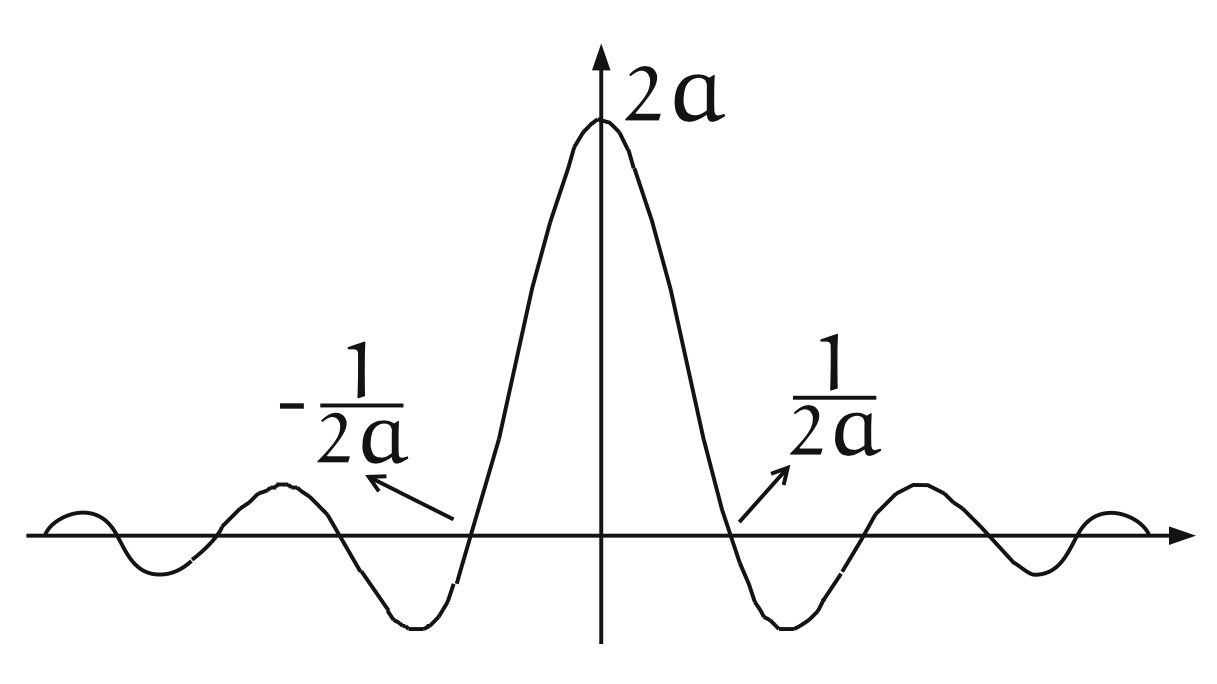
\includegraphics[width=\textwidth]{img/ch2/sinc.png}
      \caption{}
  \end{subfigure}
  \begin{subfigure}[b]{0.32\textwidth}
      \centering
      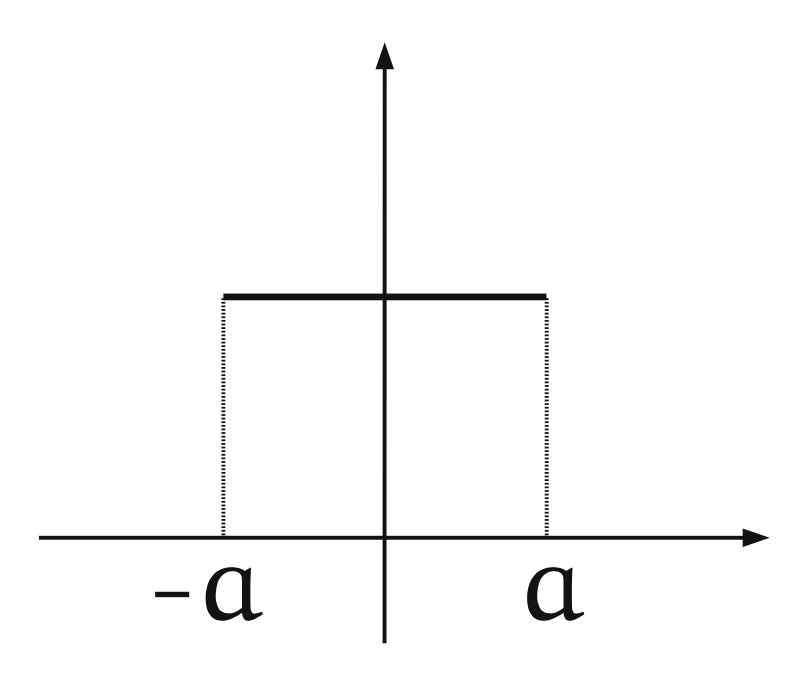
\includegraphics[width=\textwidth]{img/ch2/box.png}
      \caption{}
  \end{subfigure}
  \caption{(A) The sinc function; (B) the box function, the Fourier transform of the sinc function~\citep{ipcgVelho2014}.}
  \label{f:sinc-and-rect}
\end{figure}


The Fourier transform not only decomposes signals into their frequency components but also links sampling theory to frequency domain analysis. Since only frequencies below the Nyquist limit are preserved during sampling, the Fourier transform helps analyzing which frequencies are captured and which might cause distortion if undersampled.

The \textbf{inverse Fourier transform} is equally important, as it allows us to reconstruct the original signal from its frequency-domain representation. If we know \( F(f) = \hat{f}(s) \), the frequency-domain signal, we can retrieve the time-domain signal \( f(t) \) by applying the inverse Fourier transform:

\begin{align}
  f(t) = F^{-1}((f)(s)) = \int_{-\infty}^{\infty} \hat{f}(s) e^{2\pi i s t} ds  
\end{align}


This operation restores the original signal by integrating over all its frequency components. The Fourier transform and its inverse create a bridge between the time and frequency domains, allowing us to switch between these perspectives.

% The inverse Fourier transform provides the foundation for reconstructing signals, just as the sinc function is used in the time domain for ideal interpolation.

When signals are sampled, we effectively multiply the original continuous signal by a sequence of Dirac delta functions (impulses). In the frequency domain, this multiplication corresponds to a convolution with a train of impulses, which leads to periodic replicas of the signal's frequency spectrum. This relationship emphasizes the importance of the Nyquist criterion: if the sampling rate is too low (below twice the highest frequency in the signal), these spectral replicas overlap, resulting in aliasing. 
% The Fourier transform enables us to clearly visualize this aliasing effect by showing how undersampling distorts the signal's frequency content.

\section{Multiresolution Analysis}

Multiresolution analysis (MRA) offers a hierarchical approach to understanding signals at different levels of detail. By breaking down signals into components that represent varying scales of resolution, MRA helps to capture both global trends and fine details. This technique leverages the way we naturally process visual information, focusing on broader patterns while also perceiving intricate details as needed.

% In MRA, signals are decomposed into a coarse approximation, which retains the broader features, and a series of detail coefficients, representing finer, localized features. 

In the formal setting of MRA, a signal \( f \in L^2(\mathbb{R}^n) \), where \( L^2(\mathbb{R}^n) \) is the space of square-integrable functions in \( n \) dimensions, is represented across different scales using nested subspaces \( V_j \). These subspaces correspond to approximations of the signal at varying resolutions, with a corresponding sequence of detail subspaces \( W_j \) that capture the differences between successive levels. Mathematically, this can be expressed as:

\[
V_{j-1} = V_j \oplus W_j
\]

where \( V_{j-1} \) represents a finer approximation of the signal, and \( W_j \) captures the detail lost in transitioning from scale \( j \) to \( j-1 \). The space \( W_j \) is orthogonal to \( V_j \), and the decomposition \( V_{j-1} = V_j \oplus W_j \) enables a precise reconstruction of the signal at scale \( j-1 \).

This approach facilitates efficient representation and processing of signals, reducing storage requirements and computational complexity by focusing on the relevant details while discarding less important information. The following sections provide an overview of two primary methods for multiresolution analysis: pyramids and wavelets.

\subsection{Pyramids: Gaussian and Laplacian}

One of the simplest and most common techniques in MRA is the use of \textit{Gaussian and Laplacian pyramids}. These pyramids represent signals at multiple resolutions, enabling efficient manipulation and analysis across scales.

A \textbf{Gaussian pyramid} is built by repeatedly downsampling a signal, after applying a low-pass filter to avoid aliasing. At each level, the signal is smoothed using a Gaussian (or other low-pass) kernel and then reduced in size by subsampling. This creates a pyramid where each level contains a coarser version of the signal, with less spatial detail than the previous level. The general formulation for constructing a Gaussian pyramid in dimension \(d\) is:

\begin{align}
  G_l(\mathbf{x}) = (G_{l-1}(\mathbf{x}) * H(\mathbf{x})) \downarrow 2
  % G_l(x, y) = (G_{l-1}(x, y) * H(x, y)) \downarrow 2
\end{align}

where:
\begin{itemize}
  % \item \( G_l(x, y) \) is the Gaussian pyramid at level \( l \).
  \item \(G_l(\mathbf{x})\) is the Gaussian pyramid at level \(l\), with \(\mathbf{x} = (x_1, x_2, \dots, x_d)\) being a coordinate in \(d\)-dimensional space.
  % \item \( H(x, y) \) is a Gaussian low-pass filter.
  \item \(H(\mathbf{x})\) is a Gaussian low-pass filter in \(d\) dimensions.
  % \item \( \downarrow 2 \) denotes downsampling by a factor of 2.
  \item \(\downarrow 2\) denotes downsampling by a factor of 2 along each dimension.
\end{itemize}
 
A \textit{Laplacian pyramid} captures the differences between consecutive levels of the Gaussian pyramid, representing the high-frequency details lost during downsampling. By subtracting the smoothed, downsampled signal from its original form, the Laplacian pyramid isolates these finer details. The relationship between the Gaussian and Laplacian pyramids is given by:

\begin{align}
  L_l(\mathbf{x}) = G_{l-1}(\mathbf{x}) - (G_l(\mathbf{x}) \uparrow 2 * H(\mathbf{x}))
  % L_l(x, y) = G_{l-1}(x, y) - (G_l(x, y) \uparrow 2 * H(x, y))
\end{align}


where:
\begin{itemize}
  % \item \( L_l(x, y) \) is the Laplacian pyramid at level \( l \).
  \item \(L_l(\mathbf{x})\) is the Laplacian pyramid at level \(l\), representing the high-frequency details.
  % \item \( \uparrow 2 \) denotes upsampling by a factor of 2.
  \item \(\uparrow 2\) denotes upsampling by a factor of 2 in each dimension.
\end{itemize} 

The original signal can be reconstructed from the Laplacian pyramid by iteratively adding the details from each level back to the coarser approximations:

\begin{align}
  G_{l-1}(\mathbf{x}) = G_l(\mathbf{x}) \uparrow 2 * H(\mathbf{x}) + L_l(\mathbf{x})
  % G_{l-1}(x, y) = G_l(x, y) \uparrow 2 * H(x, y) + L_l(x, y)  
\end{align}

By progressively adding the finer details back to the lower-resolution versions, the full-resolution signal is restored. In applications like image compression, storing only the coarse approximation and the detail coefficients provides an efficient representation of the data.

\subsection{Wavelet Transforms}

While pyramid structures provide a basic form of multiresolution analysis, \textbf{wavelet transforms} offer a more sophisticated and flexible framework. Wavelets differ from pyramids in that they allow for localized multiresolution analysis in both natural and frequency domains. This makes them especially useful for signals with transient or localized features.


The key idea behind wavelets is to decompose a signal into a series of \textit{scaled} and \textit{shifted} versions of a fundamental waveform, known as the \textit{mother wavelet}. This process captures both the frequency and location information of the signal components, providing a time-frequency representation that is more adaptive than Fourier-based methods.

In wavelet analysis, a signal is decomposed into \textit{approximation coefficients}, that capture the low-frequency or smooth components of the signal, and \textit{detail coefficients}, that capture the high-frequency or detailed components, which correspond to the signal's sharp changes or fine features. This decomposition is achieved by convolving the signal with a pair of low-pass and high-pass filters. The process is applied recursively to the approximation coefficients, creating a hierarchical, multiresolution representation of the signal. The wavelet decomposition can be expressed as:

\begin{align}
  % A_l = (A_{l-1} * \phi) \downarrow 2, \quad D_l = (A_{l-1} * \psi) \downarrow 2
  A_l(\mathbf{x}) = \left( A_{l-1}(\mathbf{x}) * \phi(\mathbf{x}) \right) \downarrow 2
  \\
  D_l(\mathbf{x}) = \left( A_{l-1}(\mathbf{x}) * \psi(\mathbf{x}) \right) \downarrow 2
\end{align}

where:
\begin{itemize}
  \item \( A_l \) represents the approximation coefficients at level \( l \).
  \item \( D_l \) represents the detail coefficients at level \( l \).
  \item \( \phi \) is the scaling function, responsible for capturing low-frequency information.
  \item \( \psi \) is the wavelet function, responsible for capturing high-frequency details.
  \item \( \downarrow 2 \) denotes downsampling by a factor of 2.
\end{itemize}

% The original signal can be reconstructed from its wavelet coefficients by reversing the decomposition process, first upsampling the approximation and detail coefficients, and then applying the inverse filters.

% \begin{align}
%   A_{l-1} = (A_l \uparrow 2 * \phi) + (D_l \uparrow 2 * \psi)  
% \end{align}

The original signal can be reconstructed from its wavelet coefficients through the inverse wavelet transform. This involves upsampling the approximation and detail coefficients from the lower resolution and applying the inverse filters. The reconstruction at level \( l-1 \) is given by:

\begin{align}
  A_{l-1}(\mathbf{x}) = \left( A_l(\mathbf{x}) \uparrow 2 * \phi(\mathbf{x}) \right) + \left( D_l(\mathbf{x}) \uparrow 2 * \psi(\mathbf{x}) \right)  
\end{align}

Here, \( \uparrow 2 \) denotes upsampling by a factor of 2. The reconstruction process is computationally efficient due to the orthogonal or biorthogonal nature of the wavelet basis, which ensures minimal redundancy in the representation.

The wavelet transform operates within a hierarchy of scale spaces \( V_j \), where each space \( V_j \) corresponds to a specific level of resolution. These spaces are nested, meaning:

\begin{align}
  \cdots \subset V_{j+1} \subset V_j \subset V_{j-1} \subset \cdots  
\end{align}

Each \( V_j \) is associated with a scaling function \( \phi \), while the detail spaces \( W_j \) are spanned by a corresponding wavelet function \( \psi \), which captures the differences between successive approximations.

For more details on Wavelets and multiresolution analysis, please refer to \cite{mallat1989theory} and \cite{GomesVelho2015FromFA}.


% \subsection{Practical Applications of Wavelets}

% The versatility and efficiency of wavelet transforms make them suitable for a variety of practical applications, including:
% - **Image compression**: Wavelets are the basis for compression algorithms like JPEG2000, which exploit the multiresolution nature of wavelets to efficiently represent image data while maintaining high quality at lower bitrates.
% - **Signal denoising**: Wavelet transforms are widely used for removing noise from signals by selectively modifying or discarding the detail coefficients associated with high-frequency noise.
% - **Feature extraction**: In tasks such as computer vision and machine learning, wavelet transforms are employed to extract meaningful features from signals or images at different scales, allowing for robust analysis across various resolutions.

% The **Fast Wavelet Transform (FWT)** further enhances the practicality of wavelets by enabling efficient computation of wavelet coefficients with a complexity of \( O(n) \), making wavelets highly scalable and suitable for real-time applications.

% In summary, wavelet transforms provide a powerful tool for multiresolution analysis, capturing both spatial and frequency-domain information. Their ability to localize features across scales makes them an essential method for signal processing, compression, and analysis across various fields.

% \subsection{The Fast Wavelet Transform}

% One of the key advantages of wavelets is the **Fast Wavelet Transform (FWT)**, an efficient algorithm that decomposes a signal into its wavelet coefficients. This algorithm leverages the recursive nature of wavelet analysis, where each level of decomposition splits the signal into approximation and detail coefficients. The FWT operates in \( O(n) \) time, making it suitable for real-time applications.

% In summary, MRA using pyramids and wavelets provides a powerful framework for analyzing signals and images across scales, capturing both coarse and fine details efficiently. This hierarchical representation is fundamental in applications such as image compression, denoising, and feature extraction in computer vision and machine learning.


\section{Neural Networks}

Artificial Neural networks are computational models inspired by the biological neural networks found in animal brains. These networks consist of interconnected units known as \textbf{artificial neurons} or \textbf{perceptrons}. Each neuron receives inputs, processes them through weighted connections, and produces an output that can be transmitted to other neurons. The output of a neuron is calculated as the weighted sum of its inputs plus a bias term, composed with a non-linear function, expressed as:

\begin{align}
  \mathbf{y} = \sigma\left(\sum_{i=1}^{n} w_i x_i + \mathbf{b}\right)
  \label{eq:nn-compute}
\end{align}

In Equation \ref{eq:nn-compute}, \(\mathbf{y}\) is the output vector; \(w_i\) are the weights; \(x_i\) are the coordinates of the input vector; \(\mathbf{b}\) is the bias vector; and \(\sigma\) is a non-linear function called \textit{activation function}.

This architecture makes it possible for neural networks to learn complex patterns and relationships within data, making them particularly effective for tasks such as image recognition and natural language processing. In fact, neural networks are universal approximators (\cite{HORNIK1989359,cybenko89}).

Weights and biases are parameters of a neural network that are updated through optimization algorithms during the training process to minimize prediction error Activation functions introduce non-linearity into the network and their choice can impact the network performance and convergence during training. Common activation functions include:

\begin{itemize}
    \item \textbf{Sigmoid}: Maps outputs to a range between 0 and 1.
    \[
    f(x) = \frac{1}{1 + e^{-x}}
    \]
    
    \item \textbf{Hyperbolic Tangent (tanh)}: Maps outputs to a range between -1 and 1.
    \[
    f(x) = \tanh(x) = \frac{e^x - e^{-x}}{e^x + e^{-x}}
    \]
    
    \item \textbf{Rectified Linear Unit (ReLU)}: Outputs zero for negative inputs and identity for positive inputs.
    \[
    f(x) = \max(0, x)
    \]
\end{itemize}

Neural networks learn through a process called \textbf{backpropagation}, which efficiently computes gradients needed for optimization. The learning, or training, process involves two main steps: 

\begin{enumerate}
    \item \textbf{Forward Pass}: Inputs are passed through the network to obtain predictions.
    \item \textbf{Backward Pass}: The error between predicted outputs and actual targets is calculated using a loss function (e.g., mean squared error or cross-entropy). The gradients of this error with respect to each weight are computed using the chain rule.
\end{enumerate}

The weights are then updated using an optimization algorithm like \textbf{gradient descent}, which adjusts weights in the direction that minimizes a loss function:

\begin{align}
  \mathbf{w} = \mathbf{w} - \eta \nabla L(\mathbf{w})  
\end{align}

where \(\mathbf{w}\) represents weights; \(\eta\) is the learning rate; and \(\nabla L(\mathbf{w})\) is the gradient of the loss function with respect to weights.

Perceptrons can be connected in a variety of ways, defining different neural networks architectures. A \textbf{Multilayer Perceptron} (MLP) is a class of artificial neural networks composed of multiple layers of perceptrons, where each layer is fully connected to the next. An MLP typically consists of an input layer, one or more hidden layers, and an output layer. Each layer applies a series of weighted transformations to its inputs, followed by a non-linear activation function.

\subsection{Depth and Capacity}


Neural networks can be classified as either \textbf{shallow} or \textbf{deep} based on the number of layers in their architecture. While there is no universally accepted threshold for distinguishing between the two, a shallow network is often understood as one with at most two layers of functional composition applied to its inputs, while networks with more layers are considered deep. Increasing the number of layers enhances the network's representational power, as each layer allows the model to capture progressively more complex features from the input data.

The \textbf{capacity} of a neural network, referring to its ability to fit a range of functions, is determined by its architectural design, including both the depth (number of layers) and the width (number of neurons per layer). High-capacity networks can learn complex patterns, while low-capacity networks may struggle to capture intricate relationships in the data. Capacity is closely related to the network's \textbf{expressive power}, which defines the range of functions the network can approximate. For example, deep networks with many hidden layers and a large number of neurons can represent more complex functions than shallow networks.

However, increased capacity introduces a trade-off with generalization. A highly expressive network may overfit the training data, learning patterns that fail to generalize to unseen data. 

% The \textbf{capacity} of a model, that is its ability to fit functions is determined by the architecture of the network, including the number of layers and the number of neurons within those layers. A network with high capacity can learn complex patterns in data, while a network with low capacity may struggle to capture the underlying relationships. The capacity of a neural network is closely linked to its \textbf{expressive power}—the range of functions it can approximate. For instance, a deep neural network with many hidden layers and neurons can represent more intricate functions than a shallow network. However, this increased capacity comes with trade-offs, particularly concerning generalization. A highly expressive model might overfit the training data, learning patterns that do not generalize well to new, unseen data, thus requiring regularization techniques to manage this balance.


\subsection{Overfitting and Underfitting}

In the context of neural networks, \textbf{overfitting} and \textbf{underfitting} ara important challenges that arise from how well the model's capacity aligns with the complexity of the data. They are closely related to how the model performs on the training set versus unseen test data.

Underfitting occurs when the model is too simplistic and lacks the capacity to learn the underlying patterns in the data. This typically happens when the network has too few layers or neurons, preventing it from capturing the complexities within the dataset. As a result, the model fails to perform well on both the training data and the test data, as it cannot even identify the basic trends present in the data.

On the other hand, overfitting happens when the model has excessive capacity, allowing it to memorize the training data instead of generalizing from it. While the model might achieve very low error on the training set, it struggles to handle new, unseen data. This occurs because the overfitted model learns specific details and noise in the training data that don't generalize to broader trends in other datasets. Overfitting leads to a situation where the model's performance on the training data is excellent, but its performance on test data is significantly worse.

These two issues can be observed through the behavior of the loss function. In underfitting, both training loss and validation loss remain high, indicating that the model is not capturing enough of the underlying structure of the data: 
% $L_{\text{train}} \gg 0 \quad \text{and} \quad L_{\text{val}} \gg L_{\text{train}}$. 

% \[
% \text{High training loss and high validation loss:} \quad L_{\text{train}} \gg 0 \quad \text{and} \quad L_{\text{val}} \gg L_{\text{train}}
% \]

\[
  L_{\text{train}} \gg 0 \quad \text{and} \quad L_{\text{val}} \gg L_{\text{train}}
\]


For overfitting, the training loss becomes very low, but the validation loss is much higher, reflecting the model's poor generalization to new data: 
\[
  L_{\text{train}} \approx 0 \quad \text{and} \quad L_{\text{val}} \gg L_{\text{train}}
\]


% $L_{\text{train}} \approx 0 \quad \text{and} \quad L_{\text{val}} \gg L_{\text{train}}$

% \[
% \text{Low training loss and high validation loss:} \quad L_{\text{train}} \approx 0 \quad \text{and} \quad L_{\text{val}} \gg L_{\text{train}}
% \]

To address these challenges, it is important to find a balance between the model's capacity and its ability to generalize. Several techniques are commonly used to combat overfitting, such as regularization, dropout, and early stopping:

\textbf{Regularization} adds a penalty term to the loss function, discouraging complex models by constraining the network's weights. This helps to reduce overfitting by preventing the model from becoming too specialized to the training data.
  
\textbf{Dropout} involves randomly deactivating a portion of the neurons during training. This technique prevents neurons from relying too heavily on one another, forcing the network to learn more robust features that generalize better.
  
\textbf{Early stopping} monitors the performance of the model on validation data during training and stops the process when performance on the validation set begins to deteriorate, thereby preventing overfitting.

For more information on deep learning, including neural networks training, please, refer to \cite{goodfellow2016deep}.

% ---

\subsection{Coordinate-Based Neural Networks}

Coordinate-based neural networks represent a change of perspective in how data is modeled and encoded, especially in spatial domains like images and signals. The central concept is to use neural networks to express data as a continuous function of spatial, temporal or spatio-temporal coordinates. By doing this, various types of signals—such as 2D images or 3D shapes—can be represented by mapping coordinates directly to the corresponding output values, like pixel colors or spatial features.

% \textbf{Implicit Neural Representations (INRs)} are a specific realization of this idea. Unlike traditional methods that rely on discrete grids (e.g., pixel arrays for images or voxel grids for 3D geometries), INRs treat signals as continuous functions. Rather than storing values at fixed, discrete points, an implicit representation defines a function:

% \[
% f: \mathbb{R}^n \to \mathbb{R}^m
% \]

% This function maps any coordinate from an \(n\)-dimensional input space to a corresponding \(m\)-dimensional output value. For instance, in the case of a 2D image, an INR would take a coordinate \((x, y)\) as input and return the RGB color value at that point:

% \[
% \text{Color} = f(x, y) = (R, G, B)
% \]

One of the advantages of this continuous representation is its flexibility—it is not restricted to any specific spatial resolution. In theory, representational networks can achieve infinite resolution, meaning they can be sampled at any desired level of detail without the limitations of traditional discrete grids. Although, according to the Information Theory, it is not possible to add more details to the representation than those that were captured in the original sample.

% Furthermore, INRs offer **efficient memory usage**. The memory required to store an implicit representation scales with the complexity of the signal rather than its spatial resolution. For complex datasets, this efficiency is crucial because traditional methods might demand excessive storage, especially when handling high-resolution data.

% The impact of implicit neural representations extends far beyond storage optimization. INRs are being utilized in several advanced applications in fields like computer graphics and computer vision:

% 1. **3D Shape Representation**: INRs can outperform traditional 3D shape representations such as meshes or point clouds. By learning continuous functions over geometric shapes, they allow for seamless deep learning-based modeling of shape priors.

% 2. **Signal Reconstruction**: INRs can be used to reconstruct missing or incomplete data in signals. For example, given a sparse set of image pixels or audio data points, the learned function can fill in the gaps, making INRs particularly valuable in scenarios where the input data is noisy or incomplete.

% 3. **Solving Partial Differential Equations (PDEs)**: Some architectures, like **Sinusoidal Representation Networks (SIRENs)**, leverage periodic activation functions such as sine functions. This choice of activations enhances the network’s ability to model complex signals, including their derivatives, making SIRENs especially suitable for solving boundary value problems associated with PDEs. The periodic nature of the activations provides an ideal framework for capturing the oscillatory behavior of solutions to such equations.

% Thus, coordinate-based neural networks and implicit neural representations represent a paradigm shift in how we approach and process spatial data. By conceptualizing signals as continuous functions instead of discrete samples, these models provide enhanced flexibility, efficiency, and power in representing complex datasets. As research in this area continues to advance, these approaches are likely to drive further innovations across a range of applications, from computer vision to graphics and beyond.

One limitation of these approaches is their difficulty in handling high-frequency signal components, which arises from the spectral bias of MLPs \citep{rahaman2018spectral}. To address this, several works have adopted the method introduced by \cite{tancik2020fourfeat}, which projects input coordinates into higher-dimensional spaces using a basis of sines and cosines, a technique known as \textit{Fourier Feature Mapping}. Another effective approach in this context is the use of sinusoidal activation functions, as demonstrated by SIREN \citep{sitzmann2019siren}, which have proven capable of capturing fine high-frequency details.


\subsection{Sinusoidal Neural Networks}

Sinusoidal neural networks are examples of coordinate-based networks in which their activation function is the sine function. As such, they bridge the gap between the spatial and spectral domains, given the close relationship of the sine function with the Fourier~basis. However, these sinusoidal neural networks have been regarded as difficult to train~\citep{taming2017}. To overcome this problem, \citet{sitzmann2019siren} proposed a sinusoidal network for signal representation called SIREN. One of the contributions of this work is an initialization scheme that guarantees stability and convergence. 

% Furthermore, it also allows modeling fine details in accordance with the signal's frequency content.

The continuous nature of the sine function is particularly useful in applications where smoothness and differentiability of the output are required, such as modeling surfaces or fields in 3D space. Also, since the derivative of the sine function is the cossine, which is a shifted sine in the domain, the network's derivative preserves its properties. This characteristic makes them suitable for solving boundary value problems, such as the Poisson equation or the Helmholtz equation.


% The use of sine functions allows sinusoidal neural networks to represent signals in both the **spatial** and **frequency** domains. Signals, especially those in fields such as audio, image processing, and computer graphics, often contain fine structures that require high-frequency components for accurate representation. A sinusoidal activation function, defined as:

% \[
% \sigma(x) = \sin(x)
% \]

% is inherently capable of generating oscillations. These oscillations enable the network to capture fine variations in data, something that traditional activations might struggle with. This characteristic makes sinusoidal neural networks ideal for tasks where precision at smaller scales is critical, such as super-resolution, texture generation, or even physics simulations.

In the next chapter, we will see that the relationship between sinusoidal networks and the frequency domain is central to understanding their expressive power. 

% Each layer of the network is defined as 
% A SIREN architecture typically defines each layer of the network as:

% \[
% y = \sin(Wx + b)
% \]

% where \(W\) represents the weight matrix, \(x\) is the input, and \(b\) is the bias term. The sine activation allows the network to approximate high-frequency components, which is especially beneficial for tasks like **implicit neural representation** (as discussed previously) and **solving partial differential equations (PDEs)**.

% This decomposition reveals that any periodic signal can be described as a combination of sinusoids of different frequencies. By using sine functions as activations, sinusoidal neural networks can directly represent the frequency components of a signal, offering the ability to capture both low-frequency (coarse) and high-frequency (fine) details. This is particularly useful when modeling signals that vary at multiple scales, as the network can flexibly adapt to different frequency ranges.

% However, training SIRENs presents unique challenges. The periodic nature of sine functions can lead to difficulties in convergence during optimization due to the presence of multiple local minima in the loss landscape. To address this issue, effective initialization schemes are crucial for ensuring stability during training. These schemes help guide the optimization process toward regions of the parameter space that facilitate learning.

